\documentclass[10pt,conference,twocolumn]{style}
%Use esse arquivo para incluir novos pacotes

\usepackage[%usado para determinar medidas
	top=1.78cm,
	bottom=1.78cm,
	left=1.65cm,
	right=1.65cm,
	headsep=0cm,
	%showframe
]{geometry}
%\usepackage[justification=centering]{caption}
\usepackage{times}
\usepackage{geometry}
\usepackage{afterpage}
\usepackage{dblfloatfix}
\usepackage{enumitem}%redefinir espacos itemize
\usepackage{graphicx}
\usepackage{longtable}
\usepackage{array}
\usepackage{url,hyperref}
\usepackage{titlesec}
\usepackage[utf8]{inputenc}
\usepackage{float}%mais controle para manipular figuras
\usepackage{caption}%manipular legenda da figura e tabela
\usepackage{mathtools}%equacoes
\usepackage[hang,flushmargin]{footmisc}
\usepackage{xcolor}
\usepackage{wrapfig} %usado para envolver figura com texto
\usepackage[portuguese]{babel}
\usepackage{fancyhdr}%criacao do cabecalho
\usepackage{etoolbox}
\usepackage[export]{adjustbox}%mais controle para ajustar tamanho da tabela
\usepackage{comment}%ambiente para comentario
\usepackage{relsize} %usado por comandos \mathlarger
\usepackage{lipsum}
\usepackage{minted}

\usepackage{amsmath}  % fórmulas
\usepackage{amsfonts} % símbolos 
\usepackage{amssymb}  % mais símbolos
\usepackage{graphicx} % figuras
\usepackage{booktabs} %tabelas

\usepackage{caption}% http://ctan.org/pkg/caption

%Referencia bibliografica
\usepackage[
	style=numeric, % default: numeric/abnt
	sorting=none,
	maxbibnames=10]{biblatex}
\addbibresource{ref.bib}

%Idioma. Use "english" para trabalhos em inglês
% \usepackage[brazil]{babel}

\usepackage{threeparttable}
\usepackage{fontawesome} % icons

\usepackage{listings}
\usepackage{xcolor}

%Ajustes na legenda da figura. Incluindo espacamento apos a legenda
\captionsetup[figure]{labelformat={default},labelsep=period,font=footnotesize, name=\footnotesize{Fig.},justification=centering,singlelinecheck=false,belowskip=0\normalbaselineskip}
%\pagenumbering{gobble}

%Ajustes na legenda da tabela. 
%\captionsetup[table]{labelformat={default},labelsep=newline,font={sc,footnotesize},justification=centering,singlelinecheck=false}
\captionsetup[table]{format=plain,labelformat=simple,labelsep=period,justification=raggedright,singlelinecheck=false,skip=0pt,font=small}

%\renewcommand{\headrulewidth}{0pt}

\makeatletter
\newcommand{\linebreakand}{%
	\baselineskip
	\end{@IEEEauthorhalign}
	\hfill\mbox{}\par
	\mbox{}\hfill\begin{@IEEEauthorhalign}
}
\makeatother


%%%%%%%%%%%%%%%%%%%%%%%%%%%%%%%%%%%%%%%%%%%%%%%%%%%%%%%%%%%%%%%%%%%%%%%%%
%    Configuracaoes de Idioma
%    Considerando babel = brazil
%%%%%%%%%%%%%%%%%%%%%%%%%%%%%%%%%%%%%%%%%%%%%%%%%%%%%%%%%%%%%%%%%%%%%%%%% 

% \addto\captionsbrazil{
%   \renewcommand{\abstractname}{Abstract}
%   \renewcommand{\figurename}{Figura}
%   \renewcommand{\tablename}{Tabela}
% }
%
% %considerando babel = english
% \addto\captionsenglish{
%   \renewcommand{\tablename}{Table}
% }

% Define custom colors for syntax highlighting
\definecolor{keywordcolor}{rgb}{0.0, 0.0, 1.0} % Blue for keywords
\definecolor{stringcolor}{rgb}{0.0, 0.5, 0.0}  % Green for strings
\definecolor{commentcolor}{rgb}{0.5, 0.5, 0.5} % Gray for comments
\definecolor{backgroundcolor}{rgb}{1, 1, 1} % Light background

% Configure listings style for C code
\lstdefinestyle{mystyle}{
	backgroundcolor=\color{white}, % Set background color
	basicstyle=\ttfamily\footnotesize,       % Font size and type
	keywordstyle=\color{keywordcolor}\bfseries, % Keywords in blue and bold
	stringstyle=\color{stringcolor},          % Strings in green
	commentstyle=\color{commentcolor}\itshape, % Comments in gray and italic
	%numbers=left,                            % Line numbers on the left
	%numberstyle=\tiny\color{gray},           % Style of line numbers
	%stepnumber=1,                            % Line number step
	%numbersep=5pt,                           % Space between line numbers and code
	tabsize=2,                               % Tab size
	breaklines=true                          % Break long lines
}

\bibliography{ref.bib}

\begin{document}

\title{Circuítos Elétricos: Fundamentos}
\author{
	\IEEEauthorblockN{Gabriel dos Santos Schmitz}
	\IEEEauthorblockA{RA 2487438, Engenharia de Computação, \\
		\faEnvelope\ gabrielzschmitz@protonmail.com}
}

\maketitle
\setlength{\textfloatsep}{0pt}  % Reduce space between figure and text
\setlength{\intextsep}{0pt}     % Remove space above/below the figure when inline
\setlength{\floatsep}{0pt}      % Remove space between floats
\section{Introdução}

Irei neste documento debruçar-me-ei sobre a Geometria Analítica desde a noção
intuitiva de tratamento geométrico até o produto misto entre vetores. Farei isto
baseando-me nos livros \citetitle{winterle2014vetores}
\cite{winterle2014vetores} e \citetitle{steimbruch1987geometria}
\cite{steimbruch1987geometria}. Conforme a bibliografia usada no curso Geometria
Analítica na UTFPR de Toledo.

\section{Fundamentos Teóricos}

Nesta seção, serão apresentados as fórmulas básicas ao entendimento do
funcionamento de um circuito. Além de apresentar conceitos importantes.

\subsection{\textbf{O que é um circuito elétrico}}

Circuito elétrico, nada mais é do que um interconexão de elementos elétricos.
Elementos esses que são os componentes que formam tal circuito.

\subsection{\textbf{Grandezas importantes}}

Aqui uma tabela demosntrando as grandezas e unidades mais importantes para o
tema tratado no documento:
\newline

\begin{table}[H]
	\centering
	\caption{Grandezas e Unidades Básicas do SI}
	\begin{tabular}{m{3cm}m{2cm}m{1.5cm}}
		\hline
		\textbf{Quantidade}       & \textbf{Unidade básica} & \textbf{Símbolo} \\
		\hline
		Comprimento               & metro                   & m                \\ \hline
		Massa                     & quilograma              & kg               \\ \hline
		Tempo                     & segundo                 & s                \\ \hline
		Corrente elétrica         & ampère                  & A                \\ \hline
		Temperatura termodinâmica & kelvin                  & K                \\ \hline
		Intensidade luminosa      & candela                 & cd               \\ \hline
		Carga                     & coulomb                 & C                \\ \hline
	\end{tabular}
\end{table}

\subsection{\textbf{Grandezas importantes}}

Sabe-se que toda matéria é formada por elementos fundamentais --- átomos,
que são contituídos por elétrons, prótons e neûtrons. Vale lembrar também da
carga \textit{e} ser \( -1.602 \times 10^{-19} \)C e que quando temos o mesmo
número de prótons e elétrons temos um átomo de carga neutra.

\subsection{\textbf{Noções básicas}}

Sendo as cargas elétricas móveis, devemos considerar o fluxo destas. Portanto
quando um fio condutor é ligado a uma bateria, as cargas positivas devem se
mover para uma direção e as negativas para a direção oposta. Por convenção o
fluxo da corrente é aquele das cargas positivas ou oposta as negativas. Conforme
Figura~\ref{fig:fig1}.

\begin{figure}[H]
	\centering
	\setlength{\fboxsep}{0pt}
	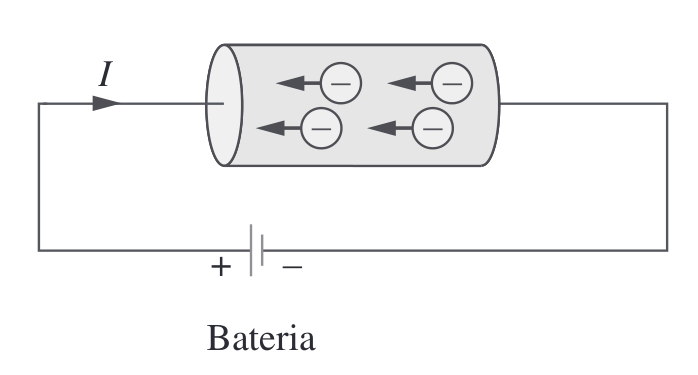
\includegraphics[height=0.1\textwidth]{./fig/fig1.png}
	\caption{Corrente elétrica devido ao fuxo de cargas eletrônicas em um condutor.}
	\label{fig:fig1}
\end{figure}

\section{Corrente Elétrica}

Corrente elétrica é o fluxo de carga por unidade de tempo, medido em ampères
(A). Matematicamente, a relação entre a corrente \textit{i}, a carga \textit{q}
e o tempo \textit{t} é:

\begin{equation}
	\label{eq:corrente}
	i \overset{\triangle}{=} \frac{dq}{dt}
\end{equation}

Onde a corrente é medida em ampères (A) e

\[
	1\,\text{ampère} = 1\,\text{coulomb}/\text{segundo}
\]

A carga transferida entre o instante \textit{\( t_0 \)} e o instante \textit{t} é
obtida integrando os dois lados da equação~\ref{eq:corrente}, onde obtemos:

\begin{equation}
	\label{eq:carga-eletrica}
	Q \overset{\triangle}{=} \int_{t_0}^{t} i\,dt
\end{equation}

\subsection{\textbf{Exemplos}}

\begin{enumerate}
	\item Qual é a quantidade de carga representada por 4600 elétrons?
	      \[
		      -1.602 \times 10^{-19} \cdot 4600 = −7.3692 \times 10^{-16}
	      \]

	\item Calcule a quantidade de carga representada por seis milhões de prótons.
	      \[
		      -1.602 \times 10^{-19} \cdot 6000000 = −9.612 \times 10^{-13}
	      \]

	\item A carga total entrando em um terminal é dada por \( q = 5t \sin{4\pi t}
	      \) mC. Calcule a corrente no instante \( t = 0.5 \) s.
	      \[
		      \begin{aligned}
			      i & = \frac{dq}{dt}                                           \\
			        & = \frac{d}{dt}\left(5t \sin{4\pi t}\right) \, \text{mC/s} \\
			        & = (5 \sin{4\pi t} + 20\pi t \cos{4\pi t}) \, \text{mA}    \\
			        & \hphantom{=} \text{para } t = 0.5                         \\
			        & = (5 \sin{2\pi} + 10\pi \cos{2\pi}) \, \text{mA}          \\
			        & = 31.42 \, \text{mA}                                      \\
		      \end{aligned}
	      \]
	\item A carga total entrando em um terminal é dada por \( q = 10 -
	      10e^{-2t} \) mC. Calcule a corrente no instante \( t = 1.0 \) s.
	      \[
		      \begin{aligned}
			      i & = \frac{dq}{dt}                                          \\
			        & = \frac{d}{dt}\left(10 - 10e^{-2t}\right) \, \text{mC/s} \\
			        & = (20e^{-2t}) \, \text{mA}                               \\
			        & \hphantom{=} \text{para } t = 1.0                        \\
			        & = (20e^{-2}) \, \text{mA}                                \\
			        & = 2.706705665 \, \text{mA}                               \\
		      \end{aligned}
	      \]
	\item Determine a carga total que entra em um terminal entre os instantes \( t
	      = 1 \) s e \( t = 2 \) s se a corrente que passa pelo terminal é \( i = (3t^2
	      – t) \) A.
	      \[
		      \begin{aligned}
			      Q & = \int_{t_0}^{t} i\,dt                            \\
			        & = \int_{1}^{2} (3t^2 - t)\,dt                     \\
			        & = \left.\left(t^3-\frac{t^2}{2}\right)\right|_1^2 \\
			        & = (8 - 2) - (1 - \frac{1}{2})                     \\
			        & = 5.5 \text{C}                                    \\
		      \end{aligned}
	      \]
	\item A corrente que fui através de um elemento é
	      \[
		      \begin{aligned}
			      i = \begin{cases}4 \text{~A},     & 0<t<1 \\
             4 t^2 \text{~A}, & t>1\end{cases} \\
		      \end{aligned}
	      \]
	      Calcule a carga que entra no elemento de \( t = 0 \) a \( t = 2 \) s.
	      \[
		      \begin{aligned}
			      Q & = \int_{0}^{2} i\,dt                                           \\
			        & = \int_{0}^{1} 4\,dt + \int_{1}^{2} 4t^2\,dt                   \\
			        & = \left[4t\right]_0^1 + \left[\frac{4t^3}{3}\right]_1^2        \\
			        & = (4(1) - 4(0)) + \left(\frac{4(8)}{3} - \frac{4(1)}{3}\right) \\
			        & = 4 + \left(\frac{32}{3} - \frac{4}{3}\right)                  \\
			        & = 4 + \frac{28}{3}                                             \\
			        & = \frac{12}{3} + \frac{28}{3}                                  \\
			        & = \frac{40}{3} \text{C} \approx 13.33333333 \,\text{C}
		      \end{aligned}
	      \]
\end{enumerate}

\subsection{\textbf{Corrente Contínua e Alternada}}

Se a corrente não muda com o tempo e permanece constante, podemos chamá-la
\textit{corrente contínua} (CC). E por convenção usa-se o símbolo \textit{I}
para representa-la.

Já se a corrente muda com o tempo, podemos chamá-la \textit{corrente alternada}
(CA). E usa-se o símbolo \textit{i} para representa-la.

\section{Tensão}

Para deslocar o elétron em um condutor determinado sentido é necessário trabalho
que é realizado por uma força eletromotriz (FEM) externa representada pela
bateria na Figura~\ref{fig:fig1}. Essa FEM também é conhecida como
\textit{tensão} ou \textit{diferença de potencial}. A tensão \( v_{ab} \) entre
dois pontos \( a \) e \( b \) em um circuito é a energia necessária para
deslocar uma carga unitária de \( a \) para \( b \); matematicamente,

\begin{equation}
	\label{eq:tensao}
	v_{ab} \overset{\triangle}{=} \frac{dw}{dq}
\end{equation}

onde \( w \) é a energia en joules (J) e \( q \) é  a carga em coulombs (C). A
tensão \( v{ab} \) ou simplesmente \( v \), é medida em volts (V). A partir da
equação~\ref{eq:tensao} fica evidente que

\[
	1\,\text{volt} = 1\,\text{joule}/\text{coulomb} = 1\,\text{newton-metro}/\text{coulomb}
\]

A Figura~\ref{fig:fig2} mostra a tensão através de um elemento conectado aos
pontos \( a \) e \( b \). Os sinais \( + \) e \( - \) são usados para definir a
polaridade da tensão. E pode ser interpretado como \( a \) esta a um pontencial
\( v_{ab} \)V mais alto que o ponto \( b \).

\begin{figure}[H]
	\centering
	\setlength{\fboxsep}{0pt}
	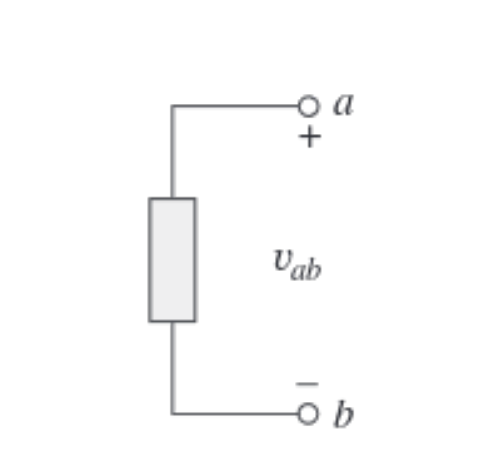
\includegraphics[height=0.15\textwidth]{./fig/fig2.png}
	\caption{Polaridade da tensão \( v_{ab} \).}
	\label{fig:fig2}
\end{figure}

Segue-se logicamente então que:

\[
	v_{ab} = -v_{ba}
\]

Uma tensão CC é comumente produzida por uma bateria e é representada por V e uma
tensão CA é produzida por um gerador elétrico sendo representada por v.

\section{Potência e Energia}

Considere, por exemplo, uma lâmpada de 100 W que fornece mais luz que uma de 60
W, ou mesmo quando pagamos nossas contas de luz às fornecedoras em que estamos
pagando pela energia elétrica consumida ao longo de certo período. Portanto, os
cálculos de potência e energia são importantes na análise de circuitos. Sendo a
potência a velocidade com que se consome ou se absorde energia, medida em
watts (W).

\begin{equation}
	\label{eq:potencia}
	p \overset{\triangle}{=} \frac{dw}{dt}
\end{equation}

onde \( p \) é a potência em watts (W), \( w \) é a energia em joules (J) e \( t
\) é o tempo em segundos (s). Sendo assim se segue que:

\begin{equation}
	\begin{aligned}
		\label{eq:potencia-instantanea}
		p & = \frac{dw}{dt}                     \\
		  & = \frac{dw}{dt} \cdot \frac{dQ}{dQ} \\
		  & = \frac{dw}{dq} \cdot \frac{dq}{dt} \\
		  & = vi                                \\
	\end{aligned}
\end{equation}

Chamada \textit{potência instantânea}, a Equação~\ref{eq:potencia-instantanea}
define que a potência é o produto da tensão no elemento pela corrente através
dele. Caso positivo esta potência é absorvida pelo elemento e caso negativa é
fornecida pelo elemento. Isto é chamado de \textit{convenção de sinal passivo} e
pode ser visualizado na Figura~\ref{fig:fig3}:

\begin{figure}[H]
	\centering
	\setlength{\fboxsep}{0pt}
	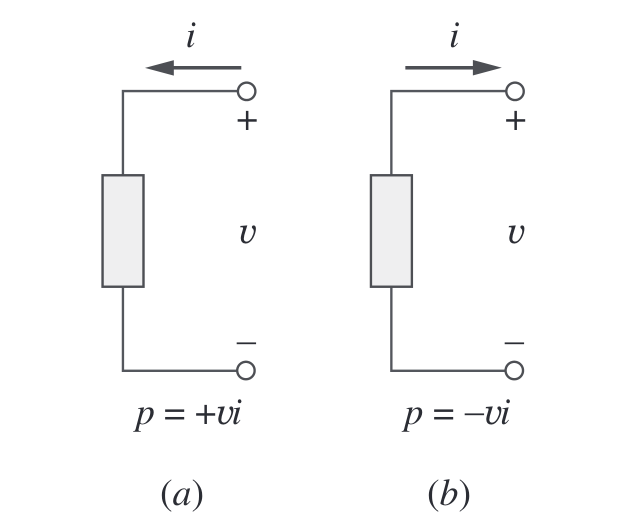
\includegraphics[height=0.15\textwidth]{./fig/fig3.png}
	\caption{Polaridades referenciais para potência usando a convenção do sinal
		passivo: (\( a \)) absorção de potência; (\( b \)) fornecimento de potência.}
	\label{fig:fig3}
\end{figure}

\[
	+\text{Potência absorvida} = –\text{Potência fornecida}
\]

Na realidade, a lei da conservação da energia tem de ser obedecida em
qualquer circuito elétrico. Por essa razão, a soma algébrica da potência em um
circuito, a qualquer instante de tempo, deve ser zero:

\[
	\sum{p} = 0
\]

A partir da Equação~\ref{eq:potencia-instantanea}, a energia absorvida ou
fornecida por um elemento do instante \( t_0 \) ao instante \( t \) é

\begin{equation}
	\begin{aligned}
		\label{eq:energia}
		w & = \int_{t_0}^t p d t   \\
		  & = \int_{t_0}^t v i d t \\
	\end{aligned}
\end{equation}

\subsection{\textbf{Exemplos}}

\begin{enumerate}
	\item Uma fonte de energia com uma corrente constante de 2 A força a passagem
	      dessa corrente através de uma lâmpada por 10 s. Se forem liberados 2,3 kJ
	      na forma de energia luminosa e calorífca, calcule a queda de tensão na
	      lâmpada.
	      \[
		      \begin{aligned}
			      \Delta q & = i \Delta t = 2 \cdot 10 = 20 \,\text{C}                          \\
			               & \hphantom{=} \text{A queda de tensão é}                            \\
			               & = \frac{\Delta w}{\Delta q} = \frac{2.3 \cdot 10^3}{20} \,\text{V} \\
			               & = 115 \,\text{V}                                                   \\
		      \end{aligned}
	      \]
	\item Mover uma carga \( q \) do ponto \( a \) ao ponto \( b \) requer –30
	      J. Determine a queda de tensão \( v_{ab} \) se: (a) \( q = 6 \) C, (b)
	      \( q = -3 \) C.
	      \begin{align*}
		      \text{(a)}\quad &
		      \begin{aligned}[t]
			      v_{ab} & = \frac{\Delta w}{\Delta q} = \frac{\lvert-30\rvert}{\lvert6\rvert} \,\text{V} \\
			             & = 5 \,\text{V}                                                                 \\
		      \end{aligned}
		      \\
		      \text{(b)}\quad &
		      \begin{aligned}[t]
			      v_{ab} & = \frac{\Delta w}{\Delta q} = \frac{\lvert-30\rvert}{\lvert-3\rvert} \,\text{V} \\
			             & = 10 \,\text{V}                                                                 \\
		      \end{aligned}
	      \end{align*}
	\item Determine a potência fornecida para um elemento no instante \( t =
	      3\) ms se a corrente que entra pelo terminal positivo for
	      \[
		      i = 5 \cos{60} \pi t \, \text{A}
	      \]
	      e a tensão for: (a) \( v = 3i \), (b) \( v = 3\frac{di}{dt} \).
	      \begin{align*}
		      \text{(a)}\quad &
		      \begin{aligned}[t]
			      \Delta p & = vi \,\text{W}                                            \\
			               & = 3i \cdot 5 \cos{60} \pi t \, \text{W}                    \\
			               & = (15 \cos{60} \pi t) \cdot (5 \cos{60} \pi t) \, \text{W} \\
			               & = 75 \cos^2{60} \pi t \, \text{W}                          \\
			               & \hphantom{=} \text{em \( t = 3 \) ms}                      \\
			               & = 75 \cos^2{60} \pi (3 \cdot 10^{-3}) \, \text{W}          \\
			               & = 75 \cos^2{0.18} \, \text{W}                              \\
			               & = 53.46672343 \,\text{W}                                   \\
		      \end{aligned}
		      \\
		      \text{(b)}\quad &
		      \begin{aligned}[t]
			      \Delta p & = vi \,\text{W}                                                      \\
			               & = 3\frac{di}{dt} \cdot 5 \cos{60} \pi t \, \text{W}                  \\
			               & = (3(-60 \pi) 5 \sin{60} \pi t) \cdot (5 \cos{60} \pi t) \, \text{W} \\
			               & = (-900 \pi \sin{60} \pi t) \cdot (5 \cos{60} \pi t) \, \text{W}     \\
			               & = -4500 \pi \sin{60} \pi t \cos{60} \pi t \, \text{W}                \\
			               & \hphantom{=} \text{em \( t = 3 \) ms}                                \\
			               & = -4500 \pi \sin{0.18} \pi \cos{0.18} \pi \, \text{W}                \\
			               & = −6395.845547 \, \text{W}                                           \\
			               & = −6.395845547 \, \text{kW}                                          \\
		      \end{aligned}
	      \end{align*}
	\item Determine a potência fornecida para o elemento no exemplo anterior no
	      instante \( t = 5\) ms se a corrente permanecer constante e a tensão
	      for: (a) \( v = 2i \), (b) \( v = (10 + 5 \int_0^t i dt) \).
	      \begin{align*}
		      \text{(a)}\quad &
		      \begin{aligned}[t]
			      \Delta p & = vi \,\text{W}                                            \\
			               & = 2i \cdot 5 \cos{60} \pi t \, \text{W}                    \\
			               & = (10 \cos{60} \pi t) \cdot (5 \cos{60} \pi t) \, \text{W} \\
			               & = 50 \cos^2{60} \pi t \, \text{W}                          \\
			               & \hphantom{=} \text{em \( t = 5 \) ms}                      \\
			               & = 50 \cos^2{60} \pi (5 \cdot 10^{-3}) \, \text{W}          \\
			               & = 17.27457514 \,\text{W}                                   \\
		      \end{aligned}
		      \\
		      \text{(b)}\quad &
		      \begin{aligned}[t]
			      \Delta p & = v i \,\text{W}                                                                                          \\
			               & = \left(10 + 5 \int_0^t i\, dt\right) \cdot 5 \cos(60\pi t) \,\text{W}                                    \\
			               & \hphantom{=} \text{em \( t = 5 \) ms}                                                                     \\
			               & = \left(10 + 5 \int_0^{0.005} 5 \cos(60\pi t)\, dt\right)                                                 \\
			               & \quad \cdot 5 \cos(60\pi \cdot 0.005) \,\text{W}                                                          \\
			               & = \left(10 + 25 \left[\frac{\sin(60\pi t)}{60\pi}\right]_0^{0.005}\right) \cdot 5 \cos(0.3\pi) \,\text{W} \\
			               & = \left(10 + \frac{25}{60\pi} [\sin(0.3\pi) - \sin(0)]\right) \cdot 5 \cdot 0.5878 \,\text{W}             \\
			               & = \left(10 + \frac{25}{60\pi} (0.8090 - 0)\right) \cdot 2.939 \,\text{W}                                  \\
			               & = \left(10 + 0.1073\right) \cdot 2.939 \,\text{W}                                                         \\
			               & = 10.1073 \cdot 2.939 \,\text{W}                                                                          \\
			               & = 29.7053547 \,\text{W}
		      \end{aligned}
	      \end{align*}
	\item Quanta energia uma lâmpada de 100 W consome em duas horas?
	      \[
		      \begin{aligned}
			      w & = pt                                                                           \\
			        & = 100 \text{W} \times 2 \text{h} \times 60 \text{min/h} \times 60 \text{s/min} \\
			        & = 720000 \, \text{J}                                                           \\
		      \end{aligned}
	      \]
	      ou:
	      \[
		      \begin{aligned}
			      w & = pt                             \\
			        & = 100 \text{W} \times 2 \text{h} \\
			        & = 200 \, \text{Wh}               \\
		      \end{aligned}
	      \]
	\item Um forno elétrico consome 15 A quando conectado a uma linha de 120 V.
	      Quanto tempo leva para consumir 180 kJ?
	      \[
		      \begin{aligned}
			      w      & = pt                 \\
			      w      & = vi t               \\
			      180000 & = 120 \cdot 15 t     \\
			      180000 & = 1800 t             \\
			      t      & = \frac{18000}{1800} \\
			      t      & = 100 \, \text{s}    \\
		      \end{aligned}
	      \]

\end{enumerate}

\section{Resistência}

No capítulo anterior, fora apresentado que aplicar uma tensão através de um fio
ou circuito resulta em um fluxo de carga ou de corrente através do fio ou do
circuito. Entretando, por que a corrente é mai intensa em alguns circuitos que
em outros? O que determina o nível de corrente resultante de uma tensão em
particular? A resposta está no fato de que há uma oposição ao fluxo de carga no
sistema que depende dos componentes do circuito, sendo este chamado
\textit{resistência}, que tem unidades \textit{ohms} (\( \Omega \)).

Essa oposição, devido fundamentalmente a colisões e fricção entre os elétrons
livres e outros elétrons, íons e átomos no curso do movimento, converte a
energia elétrica fornecida em \textit{calor}. Estas interações termodinâmicas
dependem do material do resistor.

Assim podemos definir a resistência como:

\begin{equation}
	\label{eq:lei-de-ohm}
	R \overset{\triangle}{=} \rho \frac{l}{A}
\end{equation}

Sendo \textit{\( \rho \)} a resistividade do material e sendo medidas a CM-\(
\Omega \)/pés, \textit{l} sendo o comprimento do fio em pés e \textit{A} a área
da seção transversal ou em termos leigos a grossura do fio e é medido na unidade
CM.\@ Pode-se melhor visualizar tais grandezas na Figura~\ref{fig:fig4}.

\begin{figure}[H]
	\centering
	\setlength{\fboxsep}{0pt}
	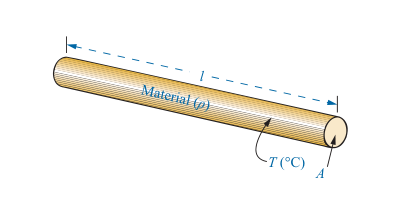
\includegraphics[height=0.15\textwidth]{./fig/fig4.png}
	\caption{Fatores que afetam a resistência de um condutor}
	\label{fig:fig4}
\end{figure}

% \[
% 	+\text{Potência absorvida} = –\text{Potência fornecida}
% \]
%
% \subsection{\textbf{Exemplos}}
%
% \begin{enumerate}
% 	\item Uma fonte de energia com uma corrente constante de 2 A força a passagem
% 	      dessa corrente através de uma lâmpada por 10 s. Se forem liberados 2,3 kJ
% 	      na forma de energia luminosa e calorífca, calcule a queda de tensão na
% 	      lâmpada.
% 	      \[
% 		      \begin{aligned}
% 			      \Delta q & = i \Delta t = 2 \cdot 10 = 20 \,\text{C}                          \\
% 			               & \hphantom{=} \text{A queda de tensão é}                            \\
% 			               & = \frac{\Delta w}{\Delta q} = \frac{2.3 \cdot 10^3}{20} \,\text{V} \\
% 			               & = 115 \,\text{V}                                                   \\
% 		      \end{aligned}
% 	      \]
% \end{enumerate}

\section{Exercícios}

Agora que tens todos os conceitos e exemplos expostos anteriormente até o
momento, chega a hora de resolver exercícios referentes aos conteúdos!

\begin{enumerate}
	\item A corrente através de um elemento é ilustrada na Figura~\ref{fig:fig5}.
	      Determine a carga total que passa pelo elemento em: (a) \( t = 1 \) s,
	      (b) \( t = 3 \) s, (c) \( t = 5 \) s.

	      \begin{figure}[H]
		      \centering
		      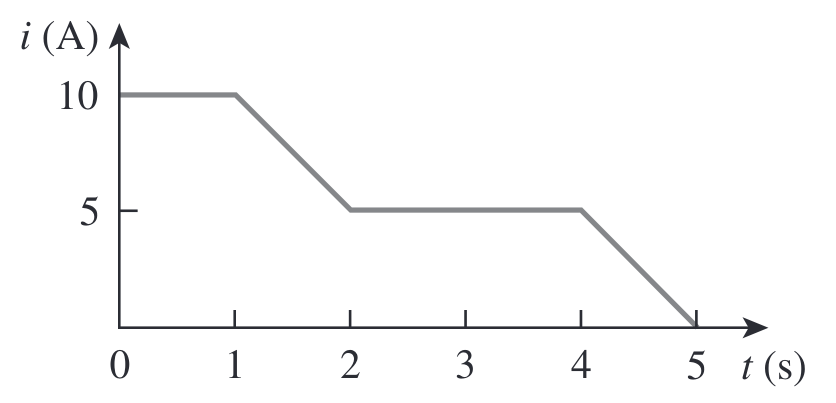
\includegraphics[height=0.15\textwidth]{./fig/fig5.png}
		      \caption{Forma de onda da corrente}
		      \label{fig:fig5}
	      \end{figure}
	      \[
		      i(t) =
		      \begin{cases}
			      10 \text{ A},            & 0 \leq t < 1 \text{ s}    \\
			      10 - 5(t - 1) \text{ A}, & 1 \leq t < 2 \text{ s}    \\
			      5 \text{ A},             & 2 \leq t < 4 \text{ s}    \\
			      5 - 6(t - 4) \text{ A},  & 4 \leq t \leq 5 \text{ s} \\
		      \end{cases}
	      \]
	      \begin{align*}
		      \text{(a)}\quad &
		      \begin{aligned}[t]
			      Q & = \int_{0}^{1} 10 \,dt = 10 \,\text{C}
		      \end{aligned}
		      \\
		      \text{(b)}\quad &
		      \begin{aligned}[t]
			      Q & = \int_{0}^{1} 10 \,dt + \int_{1}^{2} (10 - 5(t-1)) \,dt + \int_{2}^{3} 5 \,dt \\
			        & = 10 + 7.5 + 5                                                                 \\
			        & = 22.5 \,\text{C}
		      \end{aligned}
		      \\
		      \text{(c)}\quad &
		      \begin{aligned}[t]
			      Q & = \int_{0}^{1} 10 \,dt + \int_{1}^{2} (10 - 5(t-1)) \,dt     \\
			        & \quad + \int_{2}^{4} 5 \,dt + \int_{4}^{5} (5 - 5(t-4)) \,dt \\
			        & = 10 + 7.5 + 10 + 2.5                                        \\
			        & = 30 \,\text{C}
		      \end{aligned}
	      \end{align*}

	      \begin{figure}[H]
		      \centering
		      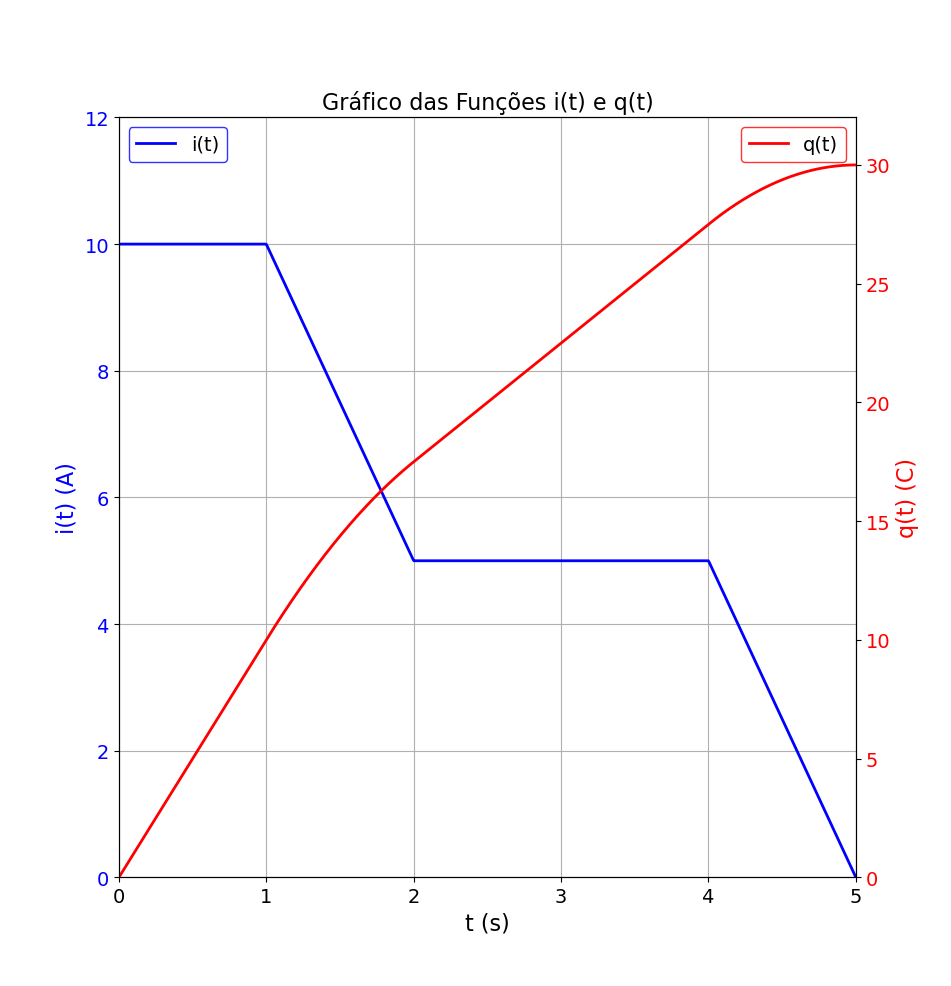
\includegraphics[height=0.425\textwidth]{./fig/fig6.png}
		      \caption{}
		      \label{fig:fig6}
	      \end{figure}
	\item A carga que entra em determinado elemento é mostrada na
	      Figura~\ref{fig:fig7}. Determine a corrente em: (a) \( t = 1 \) ms, (b)
	      \( t = 6 \) ms, (c) \( t = 10 \) ms,
	      \begin{figure}[H]
		      \centering
		      \setlength{\fboxsep}{0pt}
		      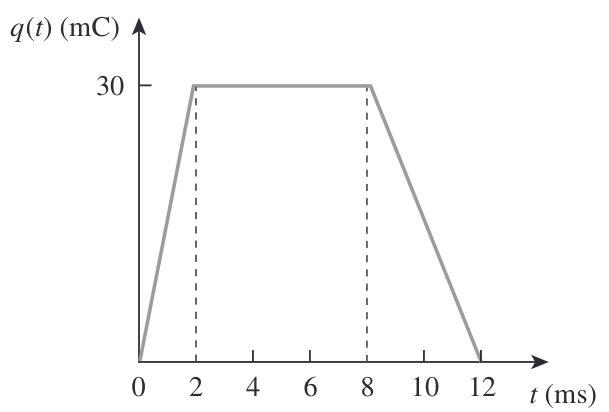
\includegraphics[height=0.2\textwidth]{./fig/fig7.png}
		      \caption{}
		      \label{fig:fig7}
	      \end{figure}
	      \begin{aligned}[t]
		      q(t) =
		      \begin{cases}
			      15t \, \text{mC},             & 0 \leq t < 2 \, \text{ms}      \\
			      30 \, \text{mC},              & 2 \leq t < 10 \, \text{ms}     \\
			      30 - 15(t - 10) \, \text{mC}, & 10 \leq t \leq 12 \, \text{ms} \\
		      \end{cases}
	      \end{aligned}
	      \vspace{6pt}
	      \begin{aligned}[t]
		      i(t) =
		      \begin{cases}
			      15 \, \text{mA},  & 0 < t < 2 \, \text{ms}   \\
			      0 \, \text{mA},   & 2 < t < 10 \, \text{ms}  \\
			      -15 \, \text{mA}, & 10 < t < 12 \, \text{ms} \\
		      \end{cases}
	      \end{aligned}
	      \vspace{6pt}
	      \begin{aligned}[t]
		      \text{(a)}\quad & i(1 \, \text{ms}) = 15 \, \text{mA}   \\
		      \text{(b)}\quad & i(6 \, \text{ms}) = 0 \, \text{mA}    \\
		      \text{(c)}\quad & i(10 \, \text{ms}) = -15 \, \text{mA} \\
	      \end{aligned}
	      \vspace{10pt}
	\item A corrente que fui por um ponto em um dispositivo é mostrada na
	      Figura~\ref{fig:fig8}. Calcule a carga total através do ponto.
	      \begin{figure}[H]
		      \centering
		      \setlength{\fboxsep}{0pt}
		      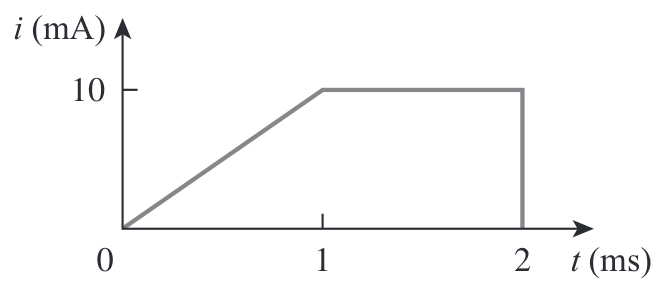
\includegraphics[height=0.15\textwidth]{./fig/fig8.png}
		      \caption{}
		      \label{fig:fig8}
	      \end{figure}
	      \begin{aligned}[t]
		      i(t) =
		      \begin{cases}
			      10t \, \text{mC}, & 0 \leq t < 1 \, \text{ms} \\
			      10 \, \text{mC},  & 1 \leq t < 2 \, \text{ms} \\
		      \end{cases}
	      \end{aligned}
	      \vspace{6pt}
	      \begin{aligned}[t]
		      Q & = \int_{0}^{1} 10t \, dt + \int_{1}^{2} 10 \, dt \\
		        & = 10 \int_{0}^{1} t \, dt + (20 - 10)            \\
		        & = 10 \frac{1}{2} \, dt + 10                      \\
		        & = 5 \, \text{mC} + 10 \, \text{mC}               \\
		        & = 15 \, \text{mC}                                \\
	      \end{aligned}
	      \newpage
	\item As Figuras~\ref{fig:fig9} e~\ref{fig:fig10} mostram a corrente e a tensão em um dispositivo.
	      \begin{enumerate}
		      \item Esboce o gráfico da potência liberada para o dispositivo para \( t > 0 \).

		            \begin{figure}[H]
			            \centering
			            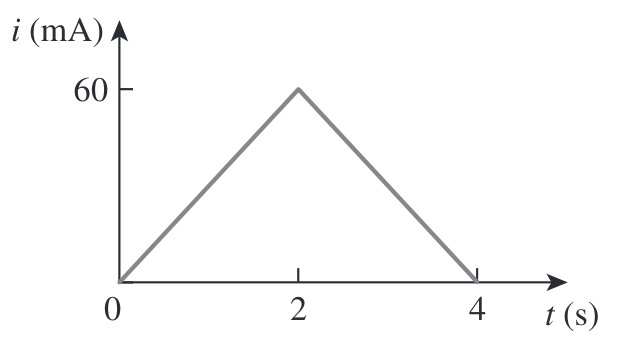
\includegraphics[height=0.15\textwidth]{./fig/fig9.png}
			            \caption{}
			            \label{fig:fig9}
		            \end{figure}
		            \begin{figure}[H]
			            \centering
			            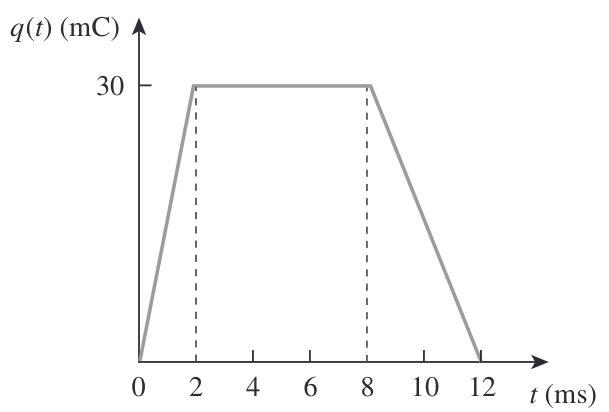
\includegraphics[height=0.15\textwidth]{./fig/fig10.png}
			            \caption{}
			            \label{fig:fig10}
		            \end{figure}

		            \begin{minipage}{\linewidth}
			            \begin{align*}
				            \rho(t)      & = v(t) \cdot i(t)                                                      \\
				            \text{Para } & 0 < t < 2 \text{ s:}                                                   \\
				            \rho(t)      & = 5 \, \text{V} \times 30t \, \text{mA} = 150t \, \text{mW}            \\
				                         & \text{\quad Potência positiva e linear (dispositivo absorve energia).} \\
				            \text{Para } & 2 \leq t \leq 4 \text{ s:}                                             \\
				            \rho(t)      & = -5 \, \text{V} \times (120 - 30t) \, \text{mA}                       \\
				                         & = -600 + 150t \, \text{mW}                                             \\
				                         & \text{\quad Potência negativa e linear (dispositivo fornece energia).} \\
			            \end{align*}
		            \end{minipage}

		            \begin{figure}[H]
			            \centering
			            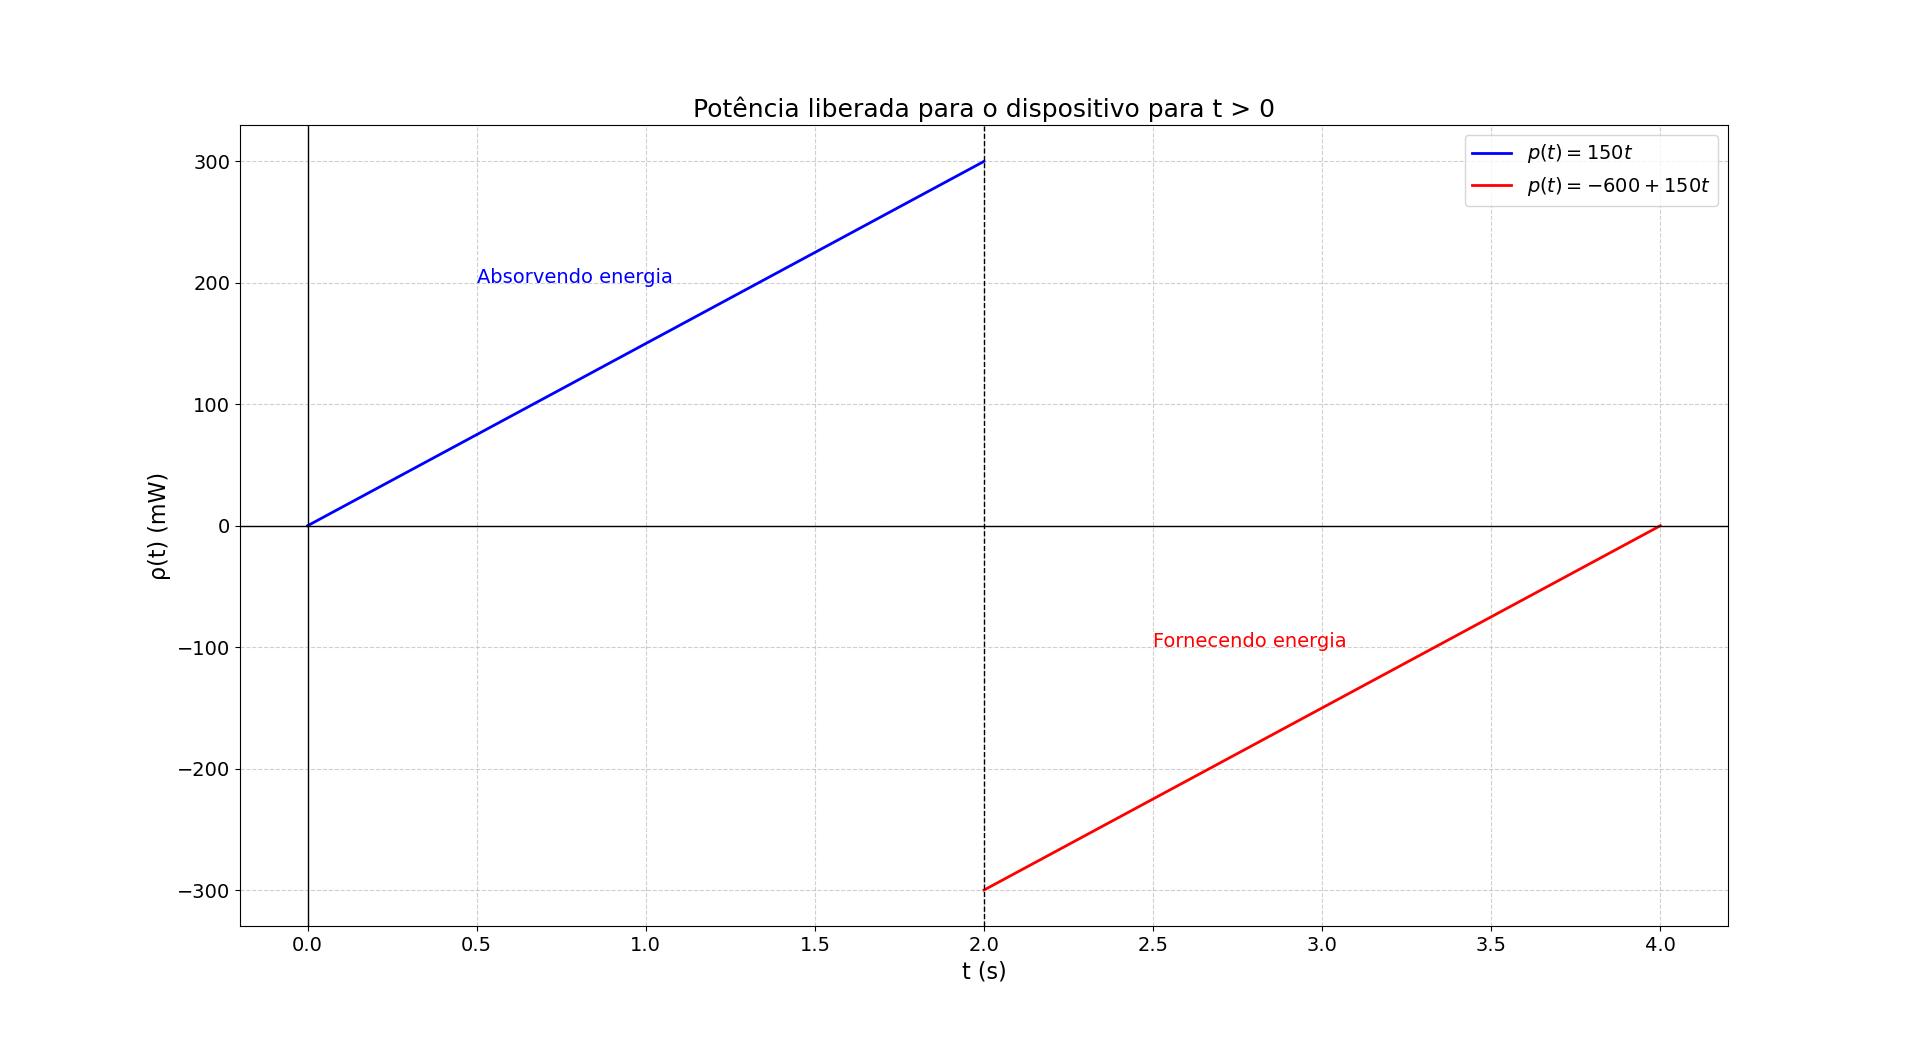
\includegraphics[height=0.325\textwidth]{./fig/fig11.png}
			            \caption{}
			            \label{fig:fig11}
		            \end{figure}

		      \item Determine a energia total absorvida pelo dispositivo para o período \( 0 < t < 4 \) s.

		            \begin{align*}
			            W & = \int_{0}^{4} p(t) \, dt                                    \\
			              & = \int_{0}^{2} 150t \, dt + \int_{2}^{4} (-600 + 150t) \, dt \\
			              & = \left[75t^2\right]_0^2 + \left[-600t + 75t^2\right]_2^4    \\
			              & = 300 \, \text{mJ} - 300 \, \text{mJ}                        \\
			              & = 0 \, \text{mJ}                                             \\
		            \end{align*}
	      \end{enumerate}
\end{enumerate}


\setlength{\bibitemsep}{10pt}
\clearpage
\onecolumn
\printbibliography\

\end{document}
